%The PDF link
\documentclass[../structure.tex]{subfiles}
%\usepackage{../mypkg}
\begin{document}
\chapter{Method and Implementation}
\section{The ICP framework}
\hspace{2em}The main subject of this thesis is demonstrating how the ICP framework can be extended to nonrigid registration, whilst keeping properties of the original algorithm. The principle idea is the application of the work presented in \cite{Amberg2007}. The extended ICP framework uses different regularisations to control the incrementally deformation of template towards the target whilst decreasing the distance and stiffness weight iteratively, recovering the whole range of global and local deformations.
\begin{comment}
To reach the goal of finding the optimal alignment of the objects (graphs), iterative closest point algorithm is used. It search for each point in the template the nearest point in target, and to find the optimal deformation for a given stiffness, optimal iterative closest point steps are used. Preliminary correspondences are estimated by a nearest point search. Subsequently, the optimal deformation of the template for these fixed correspondences and the active stiffness is calculated. Afterwards, the process continues with new correspondences found by searching from the displaced template vertices. We present an algorithm using a locally affine regularisation which assigns an affine transformation to each vertex and minimises the difference in the transformation of neighbouring vertices. It is shown that for this regularisation, the optimal deformation for fixed correspondences and fixed stiffness can be determined exactly and efficiently. The method is successful for a wide range of initial conditions. Furthermore, it is compared qualitatively and quantitatively to other algorithms using synthetic examples and real world data.
\end{comment}

\hspace{2em}As has been defined in the introduction, vertex registration is a problem in which two or more datasets of points are given and the task is to optimally align them by estimating a best transformation. In our case, we use a dense registration method to find a mapping from each point in the template onto the target while sparse methods find correspondence only for selected feature points. This is done by deforming the template, locally moving it closer in each iteration to the target in order to wrap them together with respect to stiffness.

\hspace{2em}ICP moves the template $S$ towards the target $T$ step by step. In each iteration, it minimizes the difference between the template $S$ and the target, $T$ as illustrated in figure \{\ref{fig:figure1}\}, to reach the minimal value by solving the main equation (\ref{equ:equation1}):

\begin{equation}
\label{equ:equation1}
||Ax-b||^2
\end{equation}

\hspace{2em}In equation (\ref{equ:equation1}) $x$ is a list of $X_i$, each $X_i$ is a $3\times4$ affine matrix which uses homogeneous coordinates $[x,y,z,1]$ in 3D Euclidean space. By stacking $X_i$ together we get matrix $x$ with size $4n\times3$  as shown in equation (\ref{equ:equation2}):

\begin{equation}
\label{equ:equation2}
X = [X_1, X_2, ... ,X_n]^T
\end{equation}

If we were to simply solve the equation (\ref{equ:equation1}) by assigning $A$ as the template and $b$ as the target, we will get exactly $Ax=b$, which means the difference between them is zero. That leads to the deforming of $A$ and a complete loss of its shape, therefore, we need to add the stiffness part to the equation that will prevent this deformation by keeping the vertices originally as close to each other as possible which we will later explain in this chapter.

\begin{figure}[h!]
\centering
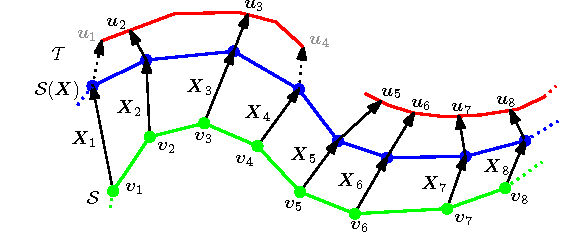
\includegraphics[scale=0.5]{001_conn}
\captionsetup{justification=centering}
\caption{The template graph $S$ (green) is deformed by locally affine transformations $(X_{i})$ onto the target graph $T$ (red). The algorithm determines closest points $(u_{i})$ for each displaced source vertex $(X_{i}v_{i})$ and finds the optimal deformation for the stiffness used in this iteration. This is repeated until a stable state is found. The process then continues with a lower stiffness. Due to the stiffness constraint the vertices do not move directly towards the target graph, but may move parallel along it. The correspondences $u_{1}$
and $u_{4}$ are dropped as they lie on the border of the target \cite{Amberg2007}.}
\label{fig:figure1}
\end{figure}

\section{Setup Data}
The method presented in \cite{Amberg2007} deals with surface graph representations of the data $S=(V,E)$ where $S,V$ and $E$ are assigned to graph, vertices and edges, respectively. As described in the introduction, our data contains human brain fiber bundles (pathways) saved in a \textbf{\textit{ply}} data format, as shown in the simplified figure \{\ref{fig:data}\}. The \textbf{\textit{ply}} format consists of three parts; the first, uppermost part is the header of the file which contains the file description (i.e. format, comment, etc) and the major components of the header element parts which describe how many elements each part has. In the sample in figure \{\ref{fig:data}\}, there are 69283 vertices in x,y,z and 603 fibers. The second part of the \textbf{\textit{ply}} files contains vertices in 3D Euclidean coordinate space while the last part of the \textbf{\textit{ply}} file represents the end index of each fiber. As the method in \cite{Amberg2007} require the template to be in graph format, we develop a tool to read \textbf{\textit{ply}} files into a numpy array of arrays which can subsequently be used as a graph. To be able to use \textbf{\textit{numpy ndarray}} as a graph, we put each tract in a separate array with respect to the link between points (Edges $E$). To do so, we put each point linked together next to each other, and then wrap all the tracts belonging to the same bundle (i.e ATR, CC, genu, splenium, etc) in a new \textbf{\textit{numpy ndarray}}.

\begin{figure}[h!]
\centering
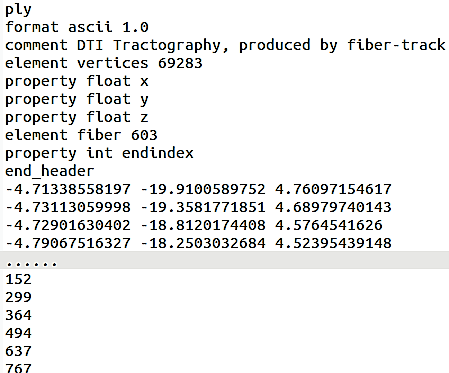
\includegraphics[scale=0.5]{002_data}
\captionsetup{justification=centering}
\caption{Simplified \textbf{\textit{ply}} file sample}
\label{fig:data}
\end{figure}

\section{Preparing graphs for ICP}
After we read the data in a graph format, we must align the template graph to the target graph as closely as possible. In order to do so, we use \textit{Principal Components Analysis (PCA)}. Before applying PCA, we scale the template graph and the target graph to a $[0,1]$ scale to match each other. This is done by subtracting all points from the minimum value in the graph and then dividing them by the maximum value in the graph. Next, we apply PCA and use $[-1,1]^3$ cube combination and measure the distance between each point in the template graph to the closest point in the target graph $\sum ||v_i-v_j||_F^2$ where $v_i \in S, v_j \in T$ eight times to select the combination with the minimum distance as is illustrated in table \{\ref{table:cube}\}.
% Above to be reviewed
\begin{center}
\begin{table}[h]
	\begin{tabular}{| c | c | c | c | c | c | c | c |}
	\hline
	1 & 2 & 3 & 4 & 5 & 6 & 7 & 8\\
	\hline
	(x,y,z) & (x,y,-z) & (x,-y,z) & (x,-y,-z) & (-x,-y,z) & (-x,y,-z) & (-x,y,z) & (-x,-y,-z)\\
	\hline
	\end{tabular}
\caption{$[-1,1]^3$ cube combination}
\label{table:cube}
\end{table}
\end{center}

\begin{figure}[h!]
	\centering
	\begin{subfigure}[b]{0.59\textwidth}
	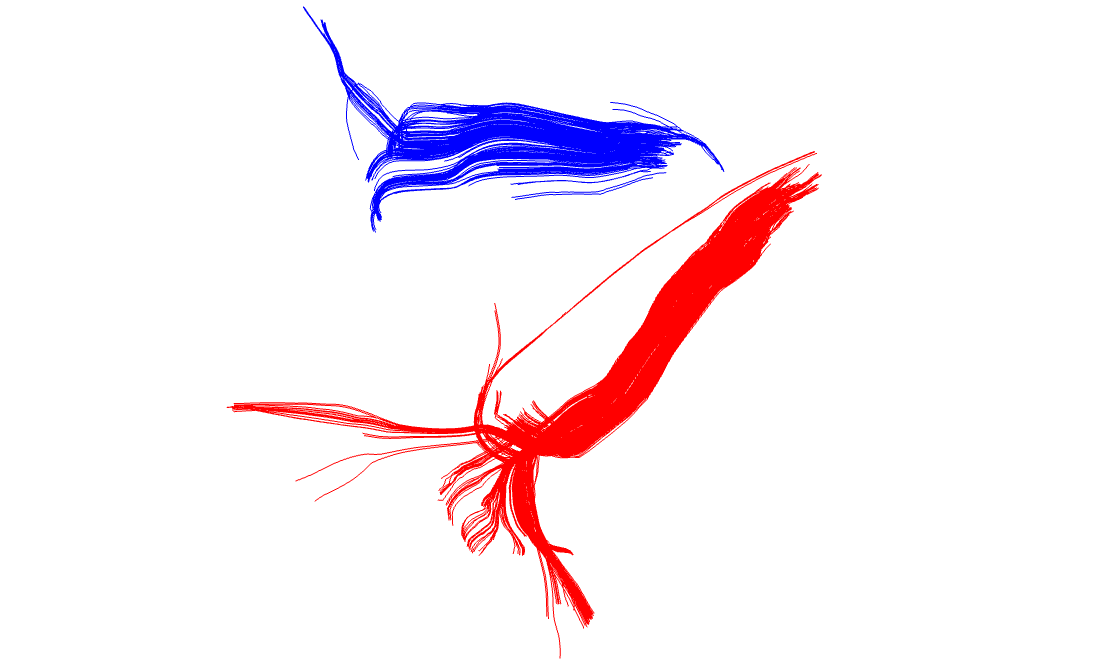
\includegraphics[width=\textwidth]{003_original}
	\caption{Original position}
	\end{subfigure}
	% separate
	\begin{subfigure}[b]{0.39\textwidth}
	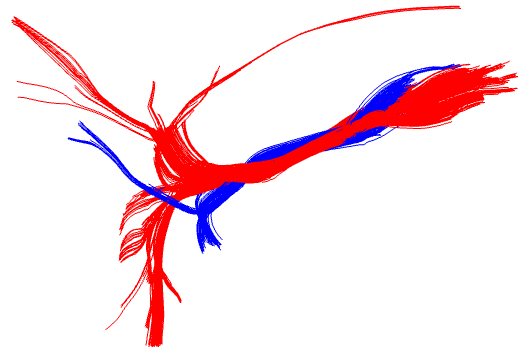
\includegraphics[width=\textwidth]{004_pca}
	\caption{After PCA}
	\end{subfigure}
\label{fig:pca}
\caption{PCA alignment}
\end{figure}

\section{Distance measurement}
In all processes in our code, we use K-D tree (or k-dimensional) to measure the euclidean distance between the points, including in PCA transformation, ICP or any other step in which we measure the distance.
\subsection{The K-D tree}
\textit{"I will right something about K-D tree"}
\begin{comment}
The K-D tree is a space-partitioning data structure (binary tree) for organizing points where every leaf node is a k-dimensional point. Every non-leaf node can be regarded as implicitly generating a splitting hyperplane that partitions the space into two parts, known as half-spaces. Points which are to the left of this hyperplane are represented by the left subtree of that node and, accordingly, points to the right of the hyperplane are represented by the right subtree. The selection of the hyperplane direction is done in the following way: each  node in the tree is associated with one of k dimensions, with the hyperplane perpendicular to that dimension's axis. For instance, if for a particular split the "x" axis is chosen, all points in the subtree with a smaller "x" value than the node will appear in the left subtree and all points with larger "x" value will be in the right subtree. In this case, the hyperplane would be set by the x-value of the point, and its normal would be the unit x-axis \cite{Bentley1975}.
\end{comment}

\begin{figure}[h!]
\centering
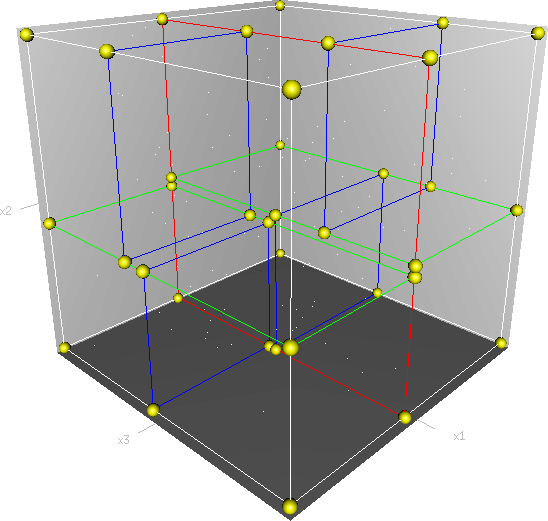
\includegraphics[scale=0.3]{005_3dtree}
\captionsetup{justification=centering}
\caption{A 3-dimensional k-d tree. The first split (the red vertical plane) cuts the root cell (white) into two subcells, each of which is then split (by the green horizontal planes) into two subcells. Finally, four cells are split (by the four blue vertical planes) into two subcells. Since there is no more splitting, the final eight are called leaf cells \cite{Wikipedia2006}.}
\label{fig:data}
\end{figure}

\section{Finding the Affine transformation Matrices}
After we prepare our data, we refer back to \cite{Amberg2007} and determine how we need to build the cost function. As we are going to explain, it consists of three parts: the distance term, stiffness term and landmark term.

As we mention above, the cost function, as shown in equation (\ref{equ:costFun}), consists of three terms, each of which represent different concepts: the distance term, stiffness term and landmark term. The distance term represents the distance between the template graph $S$ and target graph $T$ which has to be as minimal as possible (i.e., which must be minimized). The stiffness term regularizes the template graph to prevent it from being exactly the target graph. The final term is the landmark term which gives the initial case for the template graph.

\begin{equation}
E(X) = E_{d}(X) + \alpha E_{s}(X) + \beta E_{t}(X)
\label{equ:costFun}
\end{equation}
%\subsubsection{The Distance Term}
%\paragraph{The Distance Term:}
Let us illustrate the first term, \textbf{the distance term}. As we mentioned before, it is the euclidean distance between points in the template graph $S$ and points in the target graph $T$, which can be written as represented in equation (\ref{equ:distance1}). This distance has to be minimized as much as possible to align the template graph $S$ to the target graph $T$ with respect to the original shape of the template graph $S$. That means we need to ensure (by using the stiffness term, which we will discuss later in this section) that all points which are close to each other stay as near to each other as possible.

\begin{equation}
E_{d}(X) = \sum_{v_{i} \in V} w_{i}dist^2(T,X_{i}v_{i})
\label{equ:distance1}
\end{equation}

In equation (\ref{equ:distance1}), $v_{i}$ represent the vertices $V$ in the template graph $S$ in homogeneous coordinate $v_{i} = [x,y,z,1]^T$,  such that they can be multiplied by  affine matrices $X_{i}$. These affine matrices are $3 \times 4$ matrices including the transformation part, as illustrated in equation (\ref{equ:equation1}). The distance between each vertex $v_{i} \in V$ in the template graph $S$ and its closest vertex $u_{i} \in U$ in target graph $T$ noted with $dist^2(T,X_{i}v_{i})$, and $w \in [0,1]$ is weight which is \textit{one} if the correspondence for this vertex $v_{i}$ is found in the target graph $S$, and \textit{zero} otherwise. This concept will let each vertex $v_{i}$ in the template graph $T$ moves toward its correspondence vertex $u_{i}$ in the target graph $T$ if it is found, otherwise, it will move with its neighbors because of the stiffness. Essentially, we use a distance threshold as a parameter to distinguish correspondences.

Now we come to the second term, \textbf{the stiffness term}, which regularizes the shape deformation, represented in equation (\ref{equ:stiffness1}):

\begin{equation}
E_{s}(X) = \sum_{i,j \in E} ||(X_{i} - X_{j})G||_{F}^2
\label{equ:stiffness1}
\end{equation}

Regularizing the deformation occurs by penalising the weighted difference of the transformations of neighbouring vertices under the Frobenius norm $||.||_{F}$ using a weighting matrix $G := diag(1, 1, 1, \gamma)$.

The parameter $\gamma$ is used to balance the rotational and skew  against translation while transforming the template graph $S$ \cite{Amberg2007}. The value of parameter $\gamma$ depends on the units of the data and on the type of deformation that shall be expressed. In our case we select it to be one as we have already scaled our data into the $[-1, 1]^3$ cube.

We use twelve parameters per vertex in $3 \times 4$ shape. This will allow us to write the cost function as a quadratic function which can be solved directly \cite{Amberg2007}.

The Frobenius norm in equation (\ref{equ:stiffness1}) defined for matrix A is demonstrated in equation (\ref{equ:stiffness2}):

\begin{equation}
||A||_{F} = \sqrt{\sum_{i=1}^m \sum_{j=1}^n |a_{ij}|^2}
\label{equ:stiffness2}
\end{equation}

By applying this equation we keep the vertices which are linked together (i.e., there is an edge between them or they are in the same tract) or neighbors close to each other.

The $\alpha$ parameter in equation (\ref{equ:costFun}) is a constant that manages the effect of the stiffness term; when it is high the neighbor vertices doesn’t move far from eachother and when it is low, a greater deformation can occur.

The final part of the equation (\ref{equ:costFun}) is the \textbf{Stiffness term} which is demonstrated in the equation below (\ref{equ:landmark1}):

\begin{equation}
E_{l}(X) = \sum_{(vi,l) \in L}||(X_{i}v_{i} - l)||^2
\label{equ:landmark1}
\end{equation}

Amberg et al.  mention the landmark initializes and guides the registration. Given a set of landmarks $L = \left\{(v_{i1},l_{1}),(v_{i2},l_{2}),...,(v_{il},l_{l})\right\}$ mapping template graph $S$ vertices $V_{i}$ into the target graph $T$ vertices $U_{i}$.

The registration can be found even without landmarks. Without landmarks, the cost function has global minima where the template is collapsed onto a point on the target surface, but the local minimum corresponding to the correct registration can be found for a wide range of initial conditions.

In our case, we use PCA transformation as the initial step to align two graphs, therefore, we omit the landmark term later on from our cost function This is considered to be a first optimization to the cost function due to a reduction of computational  effort and time to calculate the landmark term in our code.

We illustrate now the cost function in more depth and transform the graphs in matrices that suit our cost function to ease implementation of the method.

The \textbf{distance term} in equation (\ref{equ:costFun}) and (\ref{equ:distance1}) become:

\begin{equation}
\bar{E}_{d}(X) = \sum_{v_{i}\in V} w_{i}||X_{i}v_{i}-u_{i}||^2
\label{equ:distance2}
\end{equation}
\begin{equation*}
= \left\|(W \otimes I_{3}) \left(
\begin{bmatrix}
X_{1} & & \\
& \ddots & \\
& & X_{n}
\end{bmatrix}
\begin{bmatrix}
v_{1} \\ \vdots \\ v_{n}
\end{bmatrix} -
\begin{bmatrix}
u_{1}\\ \vdots \\ u_{n}
\end{bmatrix}
\right) \right\|^2
\end{equation*}

where $W = diag(w_{1},\dots, w_{n})$ corresponds to the weight in the diagonal matrix multiplied by Kronecker product $\otimes$ to $I_{3}$ identity matrix. $X$ is diagonal matrix of $X_{i}$ that we need to solve and that is multiplied by $V$ which are vertices of template graph $S$, subtracted by the corresponding vertices $U$ of the target graph $T$.

the \textbf{Kronecker product}, denoted by $\otimes$, is an operation on two matrices of arbitrary size resulting in a block matrix. It is a generalization of the outer product, (denoted by the same symbol) from vectors to matrices, and gives the matrix of the tensor product with respect to a standard choice of basis \cite{Wikipedia2019}.

For instance, If $A$ is an $m \times n$ matrix and $B$ is a $p \times q$ matrix, then the Kronecker product $A \otimes B$ is the $mp \times nq$ block matrix:

\begin{equation*}
A \otimes B =
\begin{bmatrix}
a_{11}B & \dots  & a_{1n}B \\
\vdots  & \ddots & \vdots  \\
a_{m1}B & \dots  & a_{mn}B
\end{bmatrix}
\end{equation*}

Thus, the result of $W \otimes I_{3}$ is a $3n\times 3n$ matrix, where matrix $X$ has size $3n\times4n$, $V$ has a shape $4n\times1$ and $U$ has shape $3n\times1$.

We continue to reform the equation to be easily differentiated by converting it into canonical form. We swap the position of the $X$ and $V$ matrices. For matrix $V$ we define a sparse matrix $D$ which contains the the vertices $v_{i} \in V$ in diagonal position as demonstrated below:
\begin{equation}
D =
\begin{bmatrix}
v_{1}^T & & & \\
& v_{2}^T & & \\
& & \ddots & \\
& & & v_{n}^T
\end{bmatrix}
\end{equation}

The new format of the equation becomes:

\begin{equation}
\bar{E}_{d}(X) = ||W(DX-U)||_{F}^2
\end{equation}

Where the matrix $W$ has size $n\times n$, the matrix $D$ has size $n\times 4n$ (vertices $v_{i}$ are in homogeneous coordinates $[x,y,z,1]^T$), $X$ has size $4n\times 3$, and $U$ doesn't change with shape $n\times 3$ (vertices $u_{i}$ are in 3D coordinate).

We continue to reform \textbf{the stiffness term} which penalises differences between the transformation matrices (affine matrices) $X$ assigned to neighboring vertices. The simplified form of the stiffness term will be:

\begin{equation}
E_{s}(X) = ||(M\otimes G)X||_{F}^2
\end{equation}

where $M$ is a node-arc incidence matrix defined for directed graphs. The number of rows in this matrix equal the number of nodes (vertices) and the number of columns equal the number of arcs (edges) on the graph and the values has to be \textit{zeros, ones and/or minus ones}. The value will be \textit{zero} if the edge on this column is not connected to the vertex on this row where the value lies. Otherwise, the value must be either $1$ or $-1$; it will be $1$ if the edge direction is coming towards the vertex and $-1$ otherwise. As illustrated in the figure \{\ref{fig:directed_graph}\}, the matrix $M$ has size $e\times n$ where $e and n$ are the number of edges and vertices respectively. $G = diag(1,1,1,y)$ is the diagonal matrix and the result of $M \otimes G$ is a matrix with size $4e \times 4n$.

\begin{figure}[h!]
\centering
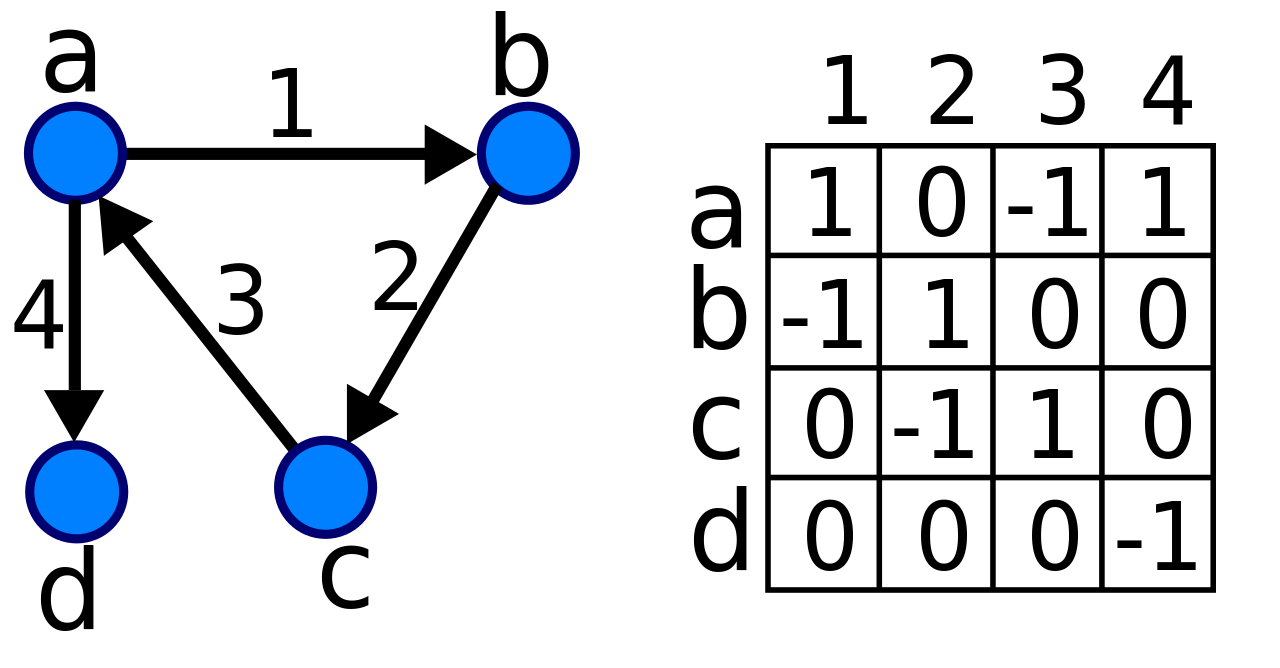
\includegraphics[scale=0.2]{006_direct_graph}
\captionsetup{justification=centering}
\caption{Oriented graph with corresponding incidence matrix  \cite{Wikipedia2010}}
\label{fig:directed_graph}
\end{figure}

The final term is \textbf{the landmark term} which needs to be reformed as well; the process of doing so is similar to that of the distance term. We only consider those vertices from $D$ ($D$ \textit{from the distance term (\ref{equ:distance2})}) which are landmarks in a new matrix called $D_{L}$, and vertices from $U$ (which are vertices from target graph $T$) which are corresponded to those landmarks. These in turn are put in a new matrix denoted $U_{L} = [l_{1}, l_{1}, \dots,l_{l}]^T$.

The final shape of the cost function is a quadratic function, as shown below:

\begin{equation}
\bar{E}(X) = \left\|
\begin{bmatrix}
\alpha M \otimes G \\ WD \\ \beta D_{L}
\end{bmatrix}
X -
\begin{bmatrix}
0 \\ WU \\ U_{L}
\end{bmatrix}
\right\| ^2 = ||AX - B||_{F}^2
\end{equation}

The current form of the function can be minimized by setting its derivative to zero and solving it as linear equation. The minimum value of $\bar{E}(X)$ is when $X = (A^T A)^{-1} A^T B$. In this case $A$ is also a sparse matrix and most of its values are zeros. However, it is still a large matrix and requires the most time in solving the equation. In order to solve the equation faster, we ommited the landmark term because we already have the initial position by applying PCA. Once we omit the landmark term, the function will be:

\begin{equation}
\bar{E}(X) = \left\|
\begin{bmatrix}
\alpha M \otimes G \\ WD
\end{bmatrix}
X -
\begin{bmatrix}
0 \\ WU
\end{bmatrix}
\right\| ^2 = ||AX - B||_{F}^2
\end{equation}

\section{Applying the Transformations}
Let us review the principle of affine transformation briefly. If we have a point $[x,y,1]$ in homogeneous coordinate in 2D euclidean space and we want to move this point three units through the \textit{X axis}, $[x,y,1]^T a = [x+3,y,1]^T$, then in this case, $a$ is called the affine matrix.

\begin{equation*}
\begin{bmatrix}
x \\ y \\ 1
\end{bmatrix}
\begin{bmatrix}
1 & 0 & 3 \\
0 & 1 & 0 \\
0 & 0 & 1
\end{bmatrix}
=
\begin{bmatrix}
x + 3 \\ y \\ 1
\end{bmatrix}
\end{equation*}

The example mentioned above is only for translation; we still have some other moves (i.e. sheer, rotation and scale) which can be performed, as demonstrated in figure \{\ref{fig:affine}\} for 2D shape.

\begin{figure}[h!]
\centering
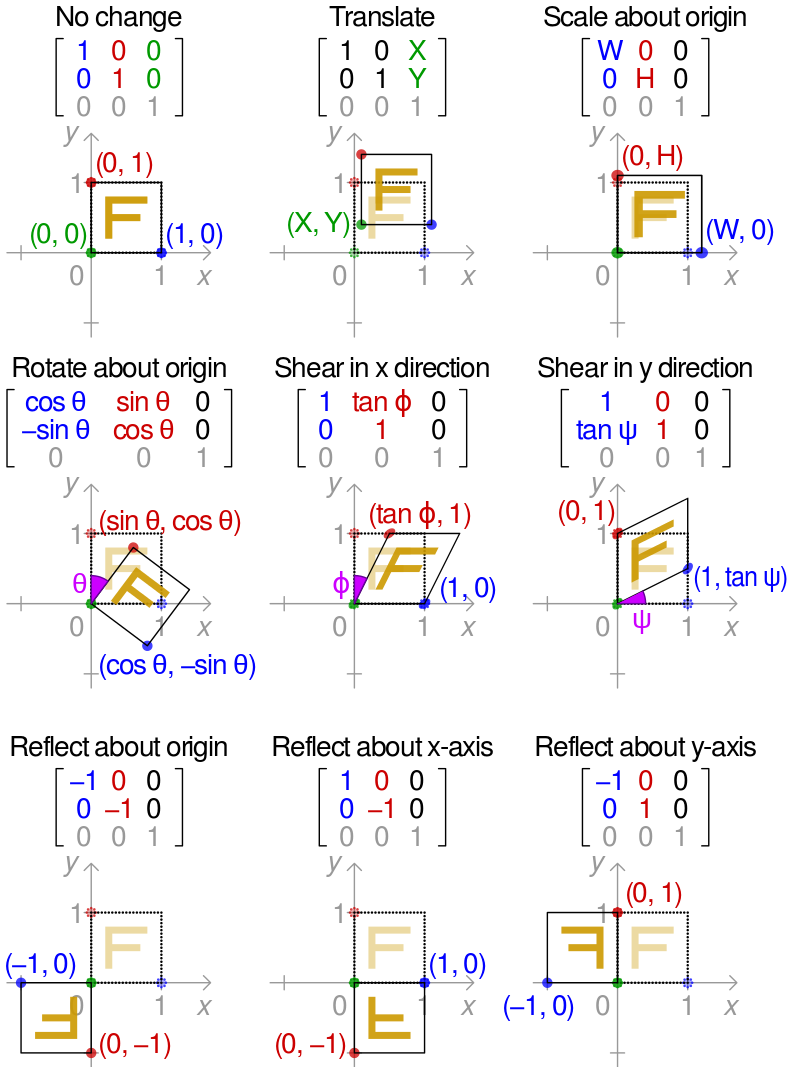
\includegraphics[scale=0.5]{007_affine}
\captionsetup{justification=centering}
\caption{2D affine transformation matrices \cite{Wikipedia2016}}
\label{fig:affine}
\end{figure}

We have shown how 2D transformation occurs; the same principles apply to 3D as well, as demonstrated below:

\begin{equation*}
\begin{bmatrix}
\hat{x} \\ \hat{y} \\ \hat{z} \\ 1
\end{bmatrix}
\begin{bmatrix}
a & b & c & e\\
f & g & h & i\\
j & k & l & m\\
0 & 0 & 0 & 1
\end{bmatrix}
=
\begin{bmatrix}
x \\ y \\ z \\ 1
\end{bmatrix}
\end{equation*}

However,  this is still for one point; if we have more points as in our case, the equation above becomes:

\begin{equation*}
\begin{bmatrix}
\hat{x_{1}} & \hat{x_{2}} & \dots & \hat{x_{n}}\\
\hat{y_{1}} & \hat{y_{2}} & \dots & \hat{y_{n}}\\
\hat{z_{1}} & \hat{z_{2}} & \dots & \hat{z_{n}}\\
1 & 1 & \dots & 1
\end{bmatrix}
\begin{bmatrix}
a & b & c & e\\
f & g & h & i\\
j & k & l & m\\
0 & 0 & 0 & 1
\end{bmatrix}
=
\begin{bmatrix}
x_{1} & x_{2} & \dots & x_{n}\\
y_{1} & y_{2} & \dots & y_{n}\\
z_{1} & z_{2} & \dots & z_{n}\\
1 & 1 & \dots & 1
\end{bmatrix}
\end{equation*}

\section{Nonrigid optimal ICP algorithms}
As we mentioned in the introduction, \textit{\textbf{ Iterative Closest Point (ICP)}} is an algorithm employed to minimize the distance between two or more points clouds. To achieve this goal, we use \textit{\textbf{Sparse Least Squares algorithm (LSQR)}} which is an iterative method for solving $Ax=b$ and $min||Ax-b||^2$, where the matrix $A$ is large and sparse (as in our case). The method is based on the bidiagonalization procedure of Golub and Kahan \cite{Paige1982a}. It is analytically equivalent to the standard method of conjugate gradients, but possesses more favorable numerical properties \cite{Paige1982a}.

We will demonstrait the idea of using \textit{LSQR} to solve our cost function in the next chapter implementation.


\section{implementation}
To implement the method we have discussed before, we wrote the code in \textit{Python Programming Language} and \textit{Spyder} version 3 and \textit{Integrated Development Environment (IDE)} are used.

As we mentioned before, our data is in \textit{\textbf{ply}} format as shown in figure \{\ref{fig:data}\}, to read this format we wrote our own method using \textit{plyfile} library due to special case of our data which has different arrangement files. The method we wrote return data in \textit{numpy ndarray} structure where each array tract is putted in an array and all tracts belong to the same bundle were putted together with respect to the sequences of the neighboring vertices.

Then we apply PCA transformation (\textit{sklearn.decomposition} library) to the data and generate histogram (\textit{matplotlib.pyplot} library) for distances between each vertex in the template graph $S$ and its closet vertex in target graph $T$, before and after PCA transformation to compare the distance difference, because in some cases where the two graphs (template and target) are already in the best alignment before ICP, PCA transformation increase the distance between them as we will show in the result chapter. If the distance between two graphs is increased we drop the PCA transformation step. For distance measurement we use \textit{K-D tree} from \textit{scikit learn}.

We continue to build variables as shown in equation (\ref{equ:finalCostFun}), to do so, we use histograms generated in the previous step to determine the threshold for the maximum distance we need to consider for $W$ in the \textbf{distance term} for cost function, if the value is equal or below the threshold $w_{i} = 1$, otherwise $w_{i} = 0$. Then we build $W$ as diaginal sparse matrix using \textit{scipy.sparse} library. Then we continue using the same library (\textit{scipy.sparse}) to build $D$ sparse matrix and calculate $WD$ and $WU$.

Now we have \textbf{the distance term} of the cost function, we need to build the \textbf{stiffness term}, we use the same library (\textit{scipy.sparse}) to build $M$ sparse matrix and $G$ diagonal sparse matrix and calculate Kronecker product ($M\otimes G$).

The final step of building the cost function is to vertically stack $MG$ and $WD$ to have $A$, and vertically stack \textit{zero} sparse matrix and $WU$ to have $B$ as require $||Ax-b||_{F}^2$.

The last step is solving the cost fuction $||Ax-b||_{F}^2$ by using \textbf{\textit{LSQR}} from \textit{scipy.sparse.linalg} library. As mentioned in the \textit{scipy.sparse.linalg.lsqr} documentation \cite{Jones2001}, $b$ in equation $Ax-b$ must be a vector, and as $b$ in our case is a matrix size $n\times 3$, we use matrices fundamental concept to solve this problem as we use \textbf{lsqrt} three times for each column and horizontally stack the result to get the affine matrices combination.

Finally for visualization we customize functions from \textit{open3d} library to view brain bundles due to special case of our data.


\begin{figure}[h!]
\centering
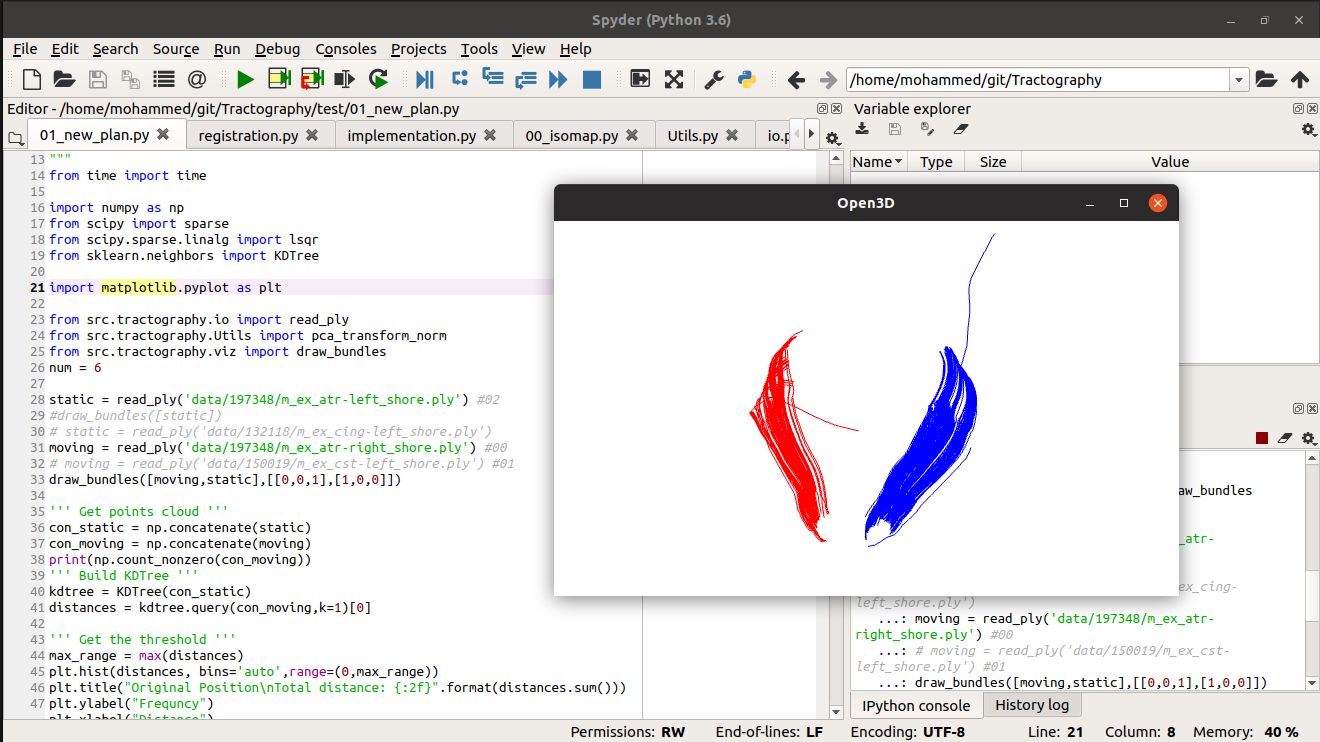
\includegraphics[scale=0.3]{008_ide}
\captionsetup{justification=centering}
\caption{IDE and visualization tool}
\end{figure}

\end{document}


